% CARA utility pages: same sample and protocol as results.tex (exp / sepalpha / commem / TK, 851 participants
% after screening out top-endpoint responders, lambda <= 20, gamma >= 0.28), exponential (CARA) utility.
% Estimates (alpha in [-0.3, 0.3]):
%   Test 3 and Test 1 C=3/C=4: results/sample_stricter_no_endpoint/cara_sepalpha_tk_wide_s500
%     (500 random starts, 250 with log-uniform alpha, screened after 20 EM iterations; warm starts incl. split C-1 fits);
%   Test 2 and Test 1 C=1/C=2: results/sample_stricter_no_endpoint/cara_sepalpha_tk_wide (100 random starts);
%   power comparison: results/sample_stricter_no_endpoint/tk_lam20_g028_main;
%   full sample: results/sample_stricter/cara_sepalpha_tk_wide and results/sample_stricter/grid (power, lambda <= 6, gamma >= 0.2);
%   alpha-bound backup: results/sample_stricter_no_endpoint/cara_sepalpha_tk (alpha <= 0.01) and 13-start scratch fits.
% Figures: python slides/make_figures.py --only cara  (writes slides/figures/cara_*.pdf)
% Compile: pdflatex results_cara.tex  (run inside slides/). The frames can also be pasted into results.tex.
\documentclass[aspectratio=169,11pt]{beamer}

\usepackage[T1]{fontenc}
\usepackage{lmodern}
\usepackage{amsmath,amssymb}
\usepackage{booktabs}
\usepackage{graphicx}

\definecolor{accent}{HTML}{2A78D6}
\definecolor{ink}{HTML}{0B0B0B}
\definecolor{muted}{HTML}{52514E}

\usetheme{default}
\setbeamertemplate{navigation symbols}{}
\setbeamertemplate{footline}[frame number]
\setbeamertemplate{itemize items}[circle]
\setbeamercolor{normal text}{fg=ink}
\setbeamercolor{structure}{fg=accent}
\setbeamercolor{frametitle}{fg=ink}
\setbeamercolor{title}{fg=ink}
\setbeamercolor{subtitle}{fg=muted}
\setbeamerfont{frametitle}{series=\bfseries}
\setbeamerfont{title}{series=\bfseries}

\graphicspath{{figures/}}

\newcommand{\ap}{\alpha^{+}}
\newcommand{\am}{\alpha^{-}}
\newcommand{\bd}{\ensuremath{^{\dagger}}}
\newcommand{\tabnote}[1]{\par\vfill{\scriptsize\color{muted}#1\par}}
\newcommand{\tight}{\setlength{\itemsep}{3pt}}
\newcommand{\rp}[1]{\rho^{#1}}

\title{Estimation Results: CARA Utility}
\date{}

\begin{document}

\begin{frame}
  \titlepage
\end{frame}

% ---------------------------------------------------------------------------
\begin{frame}{new CARA spec}


\textbf{Value function}
\begin{itemize}\small\tight
  \item Gains $\dfrac{1-e^{-\ap z}}{\ap}$, losses $-\lambda\,\dfrac{1-e^{-\am z}}{\am}$, with $z=|x-R|$ (linear at $\alpha=0$)
  \item $\alpha$ is absolute risk aversion per \pounds: $\ap>0$ is risk averse over gains, $\am>0$ risk seeking over losses
  \item $\ap,\am\in[-0.3,\,0.3]$: about the widest range floating point allows at the largest stakes
  \item Everything else as in the main specification: same 851 participants, reference points, discounting, $\gamma\ge 0.28$, $\lambda\le 20$
\end{itemize}


\tabnote{Remaining payoffs range from $-$\pounds 2{,}010 to \pounds 2{,}155 (median spread \pounds 52); $\exp(\alpha z)$ overflows beyond $|\alpha|\approx 0.33$ at these stakes. Only exponential discounting is estimated under CARA.}
\end{frame}


% ---------------------------------------------------------------------------
\begin{frame}{CARA: Test 1 ($C=1$) v.s. Test 2}
{\centering\footnotesize
\begin{tabular}{l rrrr r}
\toprule
& \multicolumn{4}{c}{Test 2: pure reference point} & Test 1\\
\cmidrule(lr){2-5}
& SQ & PA & LE & FE & weighted\\
\midrule
Log-lik. & $-71{,}659.9$ & $\mathbf{-71{,}647.2}$ & $-71{,}663.0$ & $-71{,}878.5$ & $-71{,}647.2$\\
$10^{3}\ap$ & $-0.39$ & $-0.39$ & $-0.42$ & 13.70 & $-0.39$\\
$10^{3}\am$ & $-0.04$ & $-0.02$ & $-0.08$ & 6.86 & $-0.02$\\
$\lambda$ & 1.196 & 1.205 & 1.200 & \textcolor{red}{0.792} & 1.205\\
$\gamma$ & 0.591 & 0.591 & 0.594 & 0.479 & 0.591\\
$\delta$ & -- & 0.669 & 1.000\bd & -- & 0.666\\

RP weights & & & & & $\textcolor{red}{(.00,1.00,.00,.00)}$\\
\bottomrule
\end{tabular}\par}
\begin{itemize}\small\tight
  \item One agent: utility almost linear, so risk attitude comes from $\gamma\approx 0.59$ and $\lambda\approx 1.2$; the free mix collapses to pure PA (power: PA 0.78 + FE 0.22)
\end{itemize}
\tabnote{\bd\ hitting the boundary. $r$ at its lower bound except under pure FE (0.048). $\rp{\pm}(100)$: risk premium of a 50/50 gamble between \pounds 0 and $\pm$\pounds 100. RP weights: SQ, PA, LE, FE.}
\end{frame}


\begin{frame}{Power utility: Test 1 ($C=1$) v.s. Test 2}
{\centering\footnotesize
\begin{tabular}{l rrrr r}
\toprule
& \multicolumn{4}{c}{Test 2: pure reference point} & Test 1\\
\cmidrule(lr){2-5}
& SQ & PA & LE & FE & free mix\\
\midrule
Log-lik. & $-71{,}665.4$ & $\mathbf{-71{,}653.6}$ & $-71{,}669.1$ & $-71{,}837.4$ & $-71{,}649.1$\\
$\ap$ & 1.058 & 1.062 & 1.058 & 1.159 & 1.040\\
$\am$ & 0.951 & 0.961 & 0.932 & 1.266 & 0.947\\
$\lambda$ & 1.831 & 1.792 & 1.985 & 0.525 & 1.729\\
$A(20)$ & 1.33 & 1.33 & 1.36 & 0.72 & 1.31\\
$\gamma$ & 0.595 & 0.593 & 0.600 & 0.349 & 0.594\\
$\delta$ & -- & 0.890 & 1.000\bd & -- & 0.444\\
RP weights & & & & & $(.00,.78,.00,.22)$\\
\bottomrule
\end{tabular}\par}

\tabnote{\bd\ hitting the boundary. $r$ at its lower bound except under pure FE (0.019). RP weights: SQ, PA, LE, FE.}
\end{frame}


% ---------------------------------------------------------------------------
\begin{frame}{CARA Test 1: free weight mix w/ 4 clusters}
\begin{columns}[T,onlytextwidth]
\begin{column}{0.47\textwidth}
\centering\footnotesize\setlength{\tabcolsep}{4pt}\renewcommand{\arraystretch}{0.95}
\begin{tabular}{l rrrr}
\toprule
Class & 1 & 2 & 3 & 4\\
Share $\pi$ & 36.3\% & 34.3\% & 18.3\% & 11.2\%\\
\midrule
$a_{SQ}$ & 0.113 & 0.000 & 0.044 & 0.151\\
$a_{PA}$ & 0.005 & 0.000 & 0.443 & \textbf{0.675}\\
$a_{LE}$ & 0.106 & 0.042 & 0.124 & 0.001\\
$a_{FE}$ & \textbf{0.776} & \textbf{0.958} & 0.389 & 0.173\\
$\delta$ & 0.200\bd & 0.987 & 1.000\bd & 0.860\\
\midrule
$10^{3}\ap$ & $-2.05$ & $-0.25$ & $-0.33$ & $-2.38$\\
$10^{3}\am$ & $-2.86$ & $-0.83$ & \textbf{95.7} & 0.21\\
$\lambda$ & 1.781 & 0.863 & 6.243 & 8.923\\
$\gamma$ & 0.458 & 0.716 & 0.662 & 0.280\bd\\
\bottomrule
\end{tabular}
\end{column}
\begin{column}{0.49\textwidth}
\begin{itemize}\small\tight
  \item \textbf{Two FE classes} (71\%): class 1 FE with some SQ and LE ($\lambda=1.78$, $\gamma=0.46$); class 2 pure FE with weaker probability weighting ($\gamma=0.72$, $A\approx 0.9$)
  \item \textbf{PA class} (class 4, 11\%): high loss aversion ($A\approx 9$) and $\gamma$ at the TK limit
  \item \textbf{Mixed class} (class 3, 18\%): no dominant reference point (PA 0.44, FE 0.39); strongly risk seeking over losses
  \item Population RP weights: SQ $0.07$, PA $0.16$, LE $0.08$, FE $0.70$ (power: $0.07$, $0.26$, $0.21$, $0.46$)
  \item The split between the two FE classes is weakly pinned down: fits within 1 log-lik.\ of this one range from 36/34\% to 45/23\% (backup)
\end{itemize}
\end{column}
\end{columns}
\tabnote{\bd\ at an estimation bound. $\alpha$ per \pounds; $r\le 0.007$ in all classes. Classes numbered by share. Best of 500 random and 14 warm starts.}
\end{frame}

% ---------------------------------------------------------------------------
\begin{frame}{CARA Test 3: 4 clusters w/ pre-defined RP (lowest BIC)}
\begin{columns}[T,onlytextwidth]
\begin{column}{0.45\textwidth}
\centering\footnotesize\setlength{\tabcolsep}{4pt}
\begin{tabular}{l rrrr}
\toprule
Type & SQ & PA & LE & FE\\
\midrule
Share $\pi$ & 15.0\% & 12.8\% & \textbf{54.2\%} & 18.0\%\\
Modal $n$ & 122 & 107 & 490 & 132\\
\midrule
$10^{3}\ap$ & $-0.95$ & $-0.92$ & $-0.67$ & $-0.43$\\
$10^{3}\am$ & \textbf{82.5} & 0.29 & $-1.68$ & $-0.66$\\
$\lambda$ & 3.961 & 3.194 & 1.203 & 0.955\\
$\gamma$ & 0.640 & 0.288 & 0.567 & 0.967\\
$\delta$ & -- & 0.838 & 0.200\bd & --\\
\bottomrule
\end{tabular}
\end{column}
\begin{column}{0.51\textwidth}
\begin{itemize}\small\tight
  \item \textbf{LE} (54\%): almost linear utility and mild loss aversion
  \item \textbf{SQ} (15\%): risk seeking over losses; 54\% of its loss-lottery CEs are top-of-list answers (PA 48\%, LE and FE 12\%)
  \item \textbf{PA} (13\%): strange (but acceptable) $\gamma$ monotonicity
  \item \textbf{FE} (18\%): very close to EUT
  \item Classification certainty: mean maximum posterior 0.86; 98\% above 0.5
\end{itemize}
\end{column}
\end{columns}
\tabnote{\bd\ at an estimation bound. $\alpha$ per \pounds. $\delta$ is not identified for the SQ and FE types; $r\le 0.001$ for all types. Top-of-list: CE equal to the best remaining outcome.}
\end{frame}

% ---------------------------------------------------------------------------
\begin{frame}{CARA: risk attitude by stake, Test 3 types}
\begin{columns}[c,onlytextwidth]
\begin{column}{0.58\textwidth}
\centering
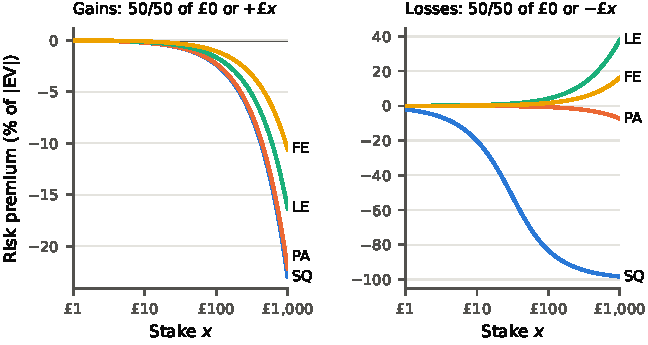
\includegraphics[width=\linewidth]{cara_risk_premium.pdf}
\end{column}
\begin{column}{0.39\textwidth}
\begin{itemize}\small\tight
  \item \textbf{Gains:} every type is mildly risk seeking: $-1.1\%$ to $-2.4\%$ at \pounds 100, $-5\%$ to $-12\%$ at \pounds 500
  \item \textbf{Losses:} SQ is strongly risk seeking; LE and FE become risk averse at large stakes ($+20\%$ and $+8\%$ at \pounds 500); PA is close to neutral
  \item Utility only: probability weighting comes on top, and gives PA most of its risk attitude ($\gamma=0.29$)
\end{itemize}
\end{column}
\end{columns}
\tabnote{$\rho(x)=(EV-CE)/|EV|$ of a 50/50 gamble between \pounds 0 and $\pm$\pounds$x$, from each type's $\ap$ or $\am$; $\lambda$ cancels. Under power utility each curve would be a flat line.}
\end{frame}

% ---------------------------------------------------------------------------
\begin{frame}{CARA: cross-test comparisons}
\begin{columns}[c,onlytextwidth]
\begin{column}{0.52\textwidth}
\centering
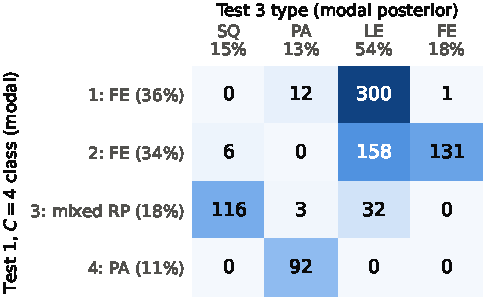
\includegraphics[width=\linewidth]{cara_crosstab_test1_test3.pdf}
\end{column}
\begin{column}{0.45\textwidth}
\begin{itemize}\small\tight
  \item \textbf{The groups match less well than under power:} 75\% of participants (639 of 851) fall in the corresponding class and type (power: 93\%)
  \item \textbf{PA and SQ} map cleanly: class 4 is the PA type (92 of 92), the mixed class 3 mostly the SQ type (116 of 151)
  \item \textbf{The two FE classes} do not separate LE from FE: class 1 is the LE type (300 of 313), class 2 splits between LE (158) and FE (131)
  \item The match depends on how the two FE classes split: the C$=4$ fit 0.86 log-lik.\ lower (45/23\%) matched 88\%
\end{itemize}
\end{column}
\end{columns}
\tabnote{Counts of participants by modal posterior class in each model; $n=851$. Classes numbered by share, as on the CARA Test 1 slide; a class is labelled by its largest RP weight if that is at least 0.6. Corresponding: best one-to-one matching of classes to types (1$\to$LE, 2$\to$FE, 3$\to$SQ, 4$\to$PA).}
\end{frame}

% ---------------------------------------------------------------------------
\begin{frame}{Power vs.\ CARA: who is which type}
\begin{columns}[c,onlytextwidth]
\begin{column}{0.48\textwidth}
\centering
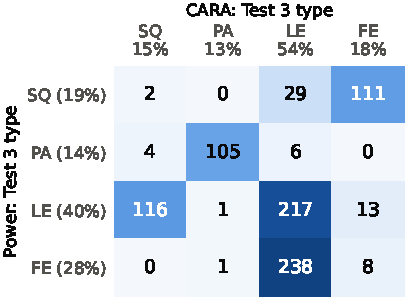
\includegraphics[width=0.92\linewidth]{cara_crosstab_utility.pdf}
\end{column}
\begin{column}{0.49\textwidth}
\begin{itemize}\small\tight
  \item \textbf{Only PA keeps its label:} 105 of the 115 power PA types are CARA PA types
  \item \textbf{The other labels move:} power FE $\to$ CARA LE (238 of 247); power SQ $\to$ CARA FE (111 of 142); power LE splits into CARA LE (217) and SQ (116)
  \item Same label for 39\% of participants; the same grouping, ignoring labels, for 67\%
  \item So the SQ, LE and FE labels depend on the utility family; the PA type does not
\end{itemize}
\end{column}
\end{columns}
\tabnote{Counts of participants by modal posterior type in each Test 3 fit; $n=851$. ``Same grouping'': best one-to-one matching of power to CARA types (SQ$\to$FE, PA$\to$PA, LE$\to$SQ, FE$\to$LE).}
\end{frame}

% ---------------------------------------------------------------------------
\begin{frame}{Full sample (1{,}081): CARA's top-of-list corner type}
\begin{columns}[T,onlytextwidth]
\begin{column}{0.50\textwidth}
\centering\footnotesize\setlength{\tabcolsep}{4pt}
\begin{tabular}{l rr}
\toprule
& Test 3 & Test 1, $C=4$\\
\midrule
BIC, power & 190{,}426.6 & 190{,}440.7\\
BIC, CARA & 189{,}838.5 & 189{,}898.8\\
\midrule
$\Delta$LL, CARA $-$ power & 294.1 & 271.0\\
\quad kept 851 & 23.9 & 60.6\\
\quad top-of-list 230 & \textbf{270.1} & \textbf{210.4}\\
\bottomrule
\end{tabular}

\vspace{8pt}
\begin{tabular}{l r}
\toprule
\multicolumn{2}{l}{CARA Test 3, FE type}\\
\midrule
Share $\pi$ / modal $n$ & 11.3\% / 116\\
Top-of-list share & $\ge 50\%$ for all, mean 84\%\\
$\ap$ / $\am$ & $-0.300$\bd\ / 0.291\\
$\lambda$ / $\gamma$ & 0.000\bd\ / 0.870\\
\bottomrule
\end{tabular}
\end{column}
\begin{column}{0.47\textwidth}
\begin{itemize}\small\tight
  \item 92\% of CARA's full-sample gain in Test 3 (270 of 294 log-lik.) comes from the 230 top-of-list participants
  \item 116 of them form the FE type: $\ap$ at its lower bound and $\lambda\to 0$, so convex gains push the CE to the best outcome and losses do not count; 77 more sit in the SQ type
  \item The bound cannot be widened ($|\alpha|<0.33$ in floating point); the FE type's $\rho^{\pm}(100)\approx-95\%$ describes the answer pattern, not risk preference
  \item Under power, 160 of them form the $\ap=5$, $\lambda=6$ corner, also at the bounds
\end{itemize}
\end{column}
\end{columns}
\tabnote{Kept: the 851 participants of the main results; top-of-list: the 230 screened out. $\Delta$LL split by participant within the same fits. Full-sample power fits use the earlier bounds $\lambda\le 6$, $\gamma\ge 0.2$; a power run with $\lambda\le 20$, $\gamma\ge 0.28$ on this sample is not available yet.}
\end{frame}

% ===========================================================================
\appendix

\begin{frame}{Backup: CARA optimisation diagnostics}
{\centering\footnotesize
\begin{tabular}{l cccc cc}
\toprule
& \multicolumn{4}{c}{Random starts within $x$ of the best log-lik.} & \multicolumn{2}{c}{Starts}\\
\cmidrule(lr){2-5}\cmidrule(lr){6-7}
Model & $x=0.01$ & $0.1$ & $1$ & $10$ & random & warm\\
\midrule
Test 2 (each RP) & 31--100 & 66--100 & 100 & 100 & 100 & 1\\
Test 1, $C=1$ & 8 & 11 & 12 & 13 & 100 & 1\\
Test 1, $C=2$ & 5 & 22 & 58 & 66 & 100 & 2\\
Test 1, $C=3$ & 1 & 1 & 22 & 40 & 214 of 500 & 6\\
Test 1, $C=4$ & \textbf{0} & \textbf{0} & 1 & 42 & 211 of 500 & 14\\
Test 3 & \textbf{0} & 2 & 3 & 17 & 208 of 500 & 2\\
\bottomrule
\end{tabular}\par}
\begin{itemize}\small\tight
  \item $C=3$, $C=4$ and Test 3: 500 random starts (250 with log-uniform $\alpha$), each screened after 20 EM iterations; the best 30\% and all warm starts run to convergence (log-lik.\ change $<10^{-6}$)
  \item $C=4$: the best fit splits a class of the $\alpha\le 0.01$ fit with $C=3$; no random start comes within 0.1 (closest: 0.21 lower, shares 41/28/19/12\%; previous best: 0.86 lower, 45/23/20/13\%)
  \item Test 3 and $C=3$: the closest random starts (0.01--0.02 and 0.13--0.14 lower) have the same shares to 0.1 percentage point
  \item At bounds: no $\alpha$ or $\lambda$; $\gamma$ only in the $C=4$ PA class; $\delta$ in several classes; $r$ at its lower bound in most classes (largest: 0.048, pure FE)
\end{itemize}
\tabnote{Random starts: finished / drawn; a random start screened out after 20 iterations is not counted. Warm starts: the same model with $\alpha\le 0.01$ (rerun: also from the 100-start run), the nested Test 3 fit and split $C-1$ fits; identical starts dropped.}
\end{frame}

\begin{frame}{Backup: the upper bound on $\alpha$}
{\centering\footnotesize
\begin{tabular}{l rr r r}
\toprule
Upper bound on $\ap,\am$ & Test 3 BIC & Test 1 ($C=4$) BIC & SQ type $\am$ & Starts\\
\midrule
0.01 & 149{,}710.1 & \textbf{149{,}536.3} & 0.010\bd & 100 + warm\\
0.03 & 149{,}544.9 & \textbf{149{,}536.3} & 0.030\bd & 13\\
0.1 & \textbf{149{,}424.3} & 149{,}456.9 & 0.083 & 13\\
0.3 (main) & \textbf{149{,}424.3} & 149{,}443.1 & 0.083 & 500 + warm\\
\bottomrule
\end{tabular}\par}
\begin{itemize}\small\tight
  \item With $\alpha\le 0.01$ or $0.03$ the SQ type sits on the bound and Test 1 ($C=4$) has the lower BIC
  \item Once $\am$ can reach 0.083, Test 3 overtakes; beyond 0.1 nothing changes
  \item The lower bound $-0.3$ does not bind on the screened sample (it does in the full sample)
\end{itemize}
\tabnote{Bold: lower BIC of the two tests. The 0.03 and 0.1 rows are 13-start checks, not full runs.}
\end{frame}

\end{document}
